% 百科创作指导

\begin{issues}
\issueTODO 
\end{issues}

\subsection{预备知识}
\begin{figure}[ht]
\centering
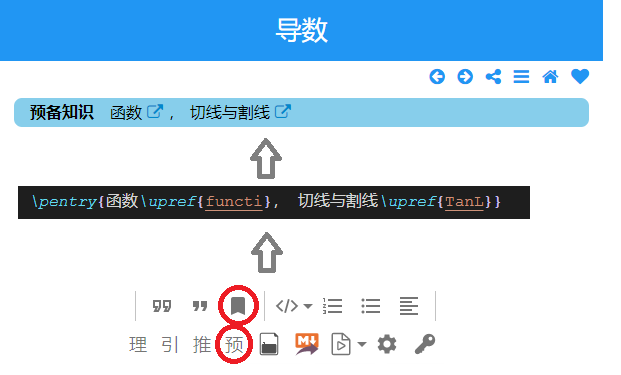
\includegraphics[width=13cm]{./figures/WrGuid_1.png}
\caption{使用菜单栏的按钮添加预备知识} \label{WrGuid_fig1}
\end{figure}

\begin{itemize}
\item 小时百科重视内容的自洽性, 所以几乎所有词条都需要指定其他一些词条作为预备知识(\autoref{WrGuid_fig1} ). 预备知识相当于 “必备知识”, 如果其中的内容不掌握, 读者阅读词条内容就会遇到较大的困难(例如从来没见过的术语,公式或定理).
\item 一般来说我们假设读者具有普通高中毕业生的数理水平. 任何超出该水平的内容都需要在 “预备知识” 中有所体现. 如果需要低于该水平的预备知识且存在相关词条, 也需要加入.
\item 注意百科词条目录并不按照建议阅读的顺序来排序而是按照话题排序, 且不鼓励读者按目录顺序阅读, 所以不能假设读者以已经读过当前词条前面的词条.
\item \href{http://wuli.wiki/tree/}{词条目录树}页面将自动按照 “预备知识” 生成. 读者可以把任意词条作为目标或起点生成该词条相关的知识树(\autoref{WrGuid_fig3} ).
\end{itemize}

\begin{figure}[ht]
\centering
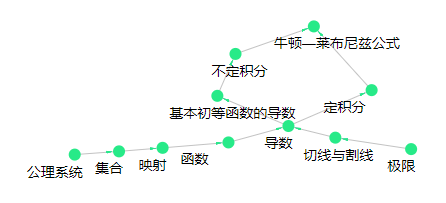
\includegraphics[width=12cm]{./figures/WrGuid_3.png}
\caption{由 “牛顿—莱布尼兹公式” 为目标生成的知识树} \label{WrGuid_fig3}
\end{figure}

\begin{itemize}
\item 注意 “预备知识” 是递归的,意味着你可以默认读者已经掌握 “预备知识” 词条中的 “预备知识”. 如果当前词条的预备知识里面已经列出了词条 A, 而词条 A 的预备知识中含有词条 B, 那么就无需把 B 再次列为当前词条的预备知识. 当然, 管理员在后台可以检测到这些重复并协助删除这些多余的预备知识.
\item 一些拓展或者选读性质的词条不需要作为预备知识, 例如 “详见……词条”.
\item 在添加预备知识时, 先浏览一下里面的内容, 确保它包含当前词条所需内容.
\item 如果百科中找不到预备知识所需的词条, 应该把当前词条标记为 “缺少预备知识” (\autoref{WrGuid_fig2}), 并用注释说明需要什么内容作为预备知识.
\end{itemize}

\begin{figure}[ht]
\centering
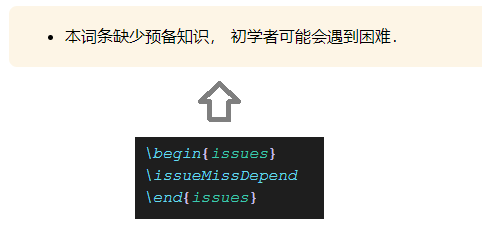
\includegraphics[width=13cm]{./figures/WrGuid_2.png}
\caption{将词条标记为 “缺少预备知识”} \label{WrGuid_fig2}
\end{figure}

\subsection{内容}
\begin{itemize}
\item 内容需要尽量对初学者友好, 例如足够的文字讲解, 图片, 例题等.
\item 如果当前内容只是一个大纲或草稿, 需要标记为草稿词条(在 \verb|issues| 环境中插入 \verb|\issueDraft|)
\item 在正文的任何地方可以用 \verb|\addTODO{}| 来插入需要补充的内容, 如果这么做, 同时需要将词条标记为 “存在未完成内容”(在 \verb|issues| 环境中插入 \verb|\issueTODO|)
\end{itemize}
\addTODO{issueAbstract, issueNeedCite, issueOther 等等}

\subsection{参考文献}
\begin{itemize}
\item 在 \verb|bibliography.tex| 的文献列表中添加你需要的参考文献, 然后在词条中用 \verb|\cite| 引用即可.
\end{itemize}
\addTODO{补充}
